%% LyX 2.1.4 created this file.  For more info, see http://www.lyx.org/.
%% Do not edit unless you really know what you are doing.
\documentclass[english]{article}
\usepackage[T1]{fontenc}
\usepackage[latin9]{inputenc}
\usepackage{amsmath}
\usepackage{amssymb}
\usepackage{graphicx}
\usepackage{babel}
\begin{document}

\title{Tightly-Coupled VI-EKF}


\author{James Jackson}

\maketitle

\section{$\boxplus$ and $\boxminus$ operators}
\begin{itemize}
\item \cite{key-1}Introduces a new syntax for working with manifold representation
of Lie Groups as if they were vectors.
\item Example: Quaternion Dynamics:
\end{itemize}
\begin{eqnarray}
\boldsymbol{q}_{t+1} & = & \boldsymbol{q}_{t}\boxplus\boldsymbol{\theta}\\
\boldsymbol{\theta} & = & \boldsymbol{q}_{1}\boxminus\boldsymbol{q}_{2}
\end{eqnarray}


It is important to note that the dimensionalities of $\boldsymbol{\theta}$
and $\boldsymbol{q}$ are different. The actual $\boxplus$ and $\boxminus$
operators are defined for robocentric quaternions representation as
follows:

\begin{align}
\boxplus & :SO\left(3\right)\times\mathbb{R}^{3}\rightarrow SO\left(3\right),\\
 & {\bf q},\boldsymbol{\theta}\mapsto{\bf q}\otimes\exp\left(\boldsymbol{\theta}\right)\\
\boxminus & :SO\left(3\right)\times SO\left(3\right)\rightarrow\mathbb{R}^{3},\\
 & {\bf q},{\bf p}\mapsto\log\left({\bf p}\otimes{\bf q}^{-1}\right),
\end{align}


This is a sort of weird syntax, but it allows us to work with these
parameterizations as if they were vectors. These operators become
the equivalent of vector addition and subtraction, and therefore allow
proper defintions of derivatives and integrals across these operators.
A properly defined $\boxplus$ manifold must obey the following identies

\begin{eqnarray}
 & x\boxplus0 & =x\\
\forall y\in S:\quad & x\boxplus\left(y\boxminus x\right) & =y\\
\forall\delta\in V:\quad & (x\boxplus\delta)\boxminus x & =\delta\\
\forall\delta_{1}\delta_{1}\in\mathbb{R}^{n}:\quad & \lVert(x\boxplus\delta_{1})\boxminus(x\boxplus\delta_{2})\rVert & \leq\lVert\delta_{1}-\delta_{2}\rVert
\end{eqnarray}


These operators must also form a diffeomorphism from $V$ to $S$,
so that derivatives of $\delta$ correspond to limits of $x\boxplus\delta$.
For example, the derivative of a quaternion, as defined using the
$\boxplus$ and $\boxminus$ operators are
\begin{eqnarray}
\dfrac{\partial}{\partial x}\boldsymbol{q}(x) & : & =\lim_{\epsilon\rightarrow0}\dfrac{\boldsymbol{q}(x+\epsilon)\boxminus\boldsymbol{q}(x)}{\epsilon}\\
\dfrac{\partial}{\partial\boldsymbol{q}}x(\boldsymbol{q}) & : & =\lim_{\epsilon\rightarrow0}\left[\begin{array}{c}
\dfrac{x\left(\boldsymbol{q}\boxplus(\boldsymbol{e}_{1}\epsilon)\right)-x\left(\boldsymbol{q}\right)}{\epsilon}\\
\dfrac{x\left(\boldsymbol{q}\boxplus(\boldsymbol{e}_{2}\epsilon)\right)-x\left(\boldsymbol{q}\right)}{\epsilon}\\
\dfrac{x\left(\boldsymbol{q}\boxplus(\boldsymbol{e}_{3}\epsilon)\right)-x\left(\boldsymbol{q}\right)}{\epsilon}
\end{array}\right]^{\top}
\end{eqnarray}


Derivatives over all $\boxplus$ and $\boxminus$ operators can be
found in a similar manner. Which allows us to use this operator to
define dynamics and Jacobians across our non-linear manifold representations.

We can represent covariance using the $\boxplus$ and $\boxminus$
operators in the following method

\begin{equation}
\mathcal{N}\left(\mu,\Sigma\right):=\mu\boxplus\mathcal{N}\left(0,\Sigma\right)
\end{equation}


It is important to note here that in many cases,
\begin{align}
\mu\in\mathbb{R}^{m}\\
\Sigma\in\mathbb{R}^{n\times n}\\
m\neq n
\end{align}



\section{Quaternions}

We will use standard Hamiltonian Notation for quaternions:

\begin{equation}
{\bf q}=q_{w}+q_{x}{\bf i}+q_{y}{\bf j}+q_{z}{\bf k}=\begin{bmatrix}\bar{{\bf q}}^{\top} & q_{w}\end{bmatrix}^{\top},
\end{equation}


where quaternion multiplication is defined as

\begin{equation}
{\bf p}\otimes{\bf q}=\begin{bmatrix}p_{w}{\bf I+\left\lfloor \bar{{\bf p}}\right\rfloor } & \bar{{\bf p}}\\
-\bar{{\bf p}}^{\top} & p_{w}
\end{bmatrix}\begin{bmatrix}\bar{{\bf q}}\\
q_{w}
\end{bmatrix},
\end{equation}


The $3\times3$ Rotation matrix based on this quaternion is defined
as follows

\begin{equation}
R\left({\bf q}\right)=\left(2q_{w}^{2}-1\right){\bf I}-2q_{w}\left\lfloor \bar{{\bf q}}\right\rfloor +2\bar{{\bf q}}\bar{{\bf q}}^{\top}\in\mathbb{R}^{3\times3}
\end{equation}


The exponential mapping used to define the $\boxplus$ and $\boxminus$
operators 

\begin{equation}
\exp\left(\boldsymbol{\delta}\right)=\begin{bmatrix}\bar{{\bf q}}\\
q_{w}
\end{bmatrix}=\begin{bmatrix}\sin\left(\frac{\lVert\delta\rVert}{2}\right)\frac{\delta}{\lVert\delta\rVert}\\
\cos\left(\frac{\lVert\delta\rVert}{2}\right)
\end{bmatrix},
\end{equation}


\begin{equation}
\log\left({\bf q}\right)=2\mathrm{atan2}\left(\left\Vert \bar{{\bf q}}\right\Vert ,q_{w}\right)\frac{\bar{{\bf q}}}{\left\Vert \bar{{\bf q}}\right\Vert },
\end{equation}


The $\boxminus$ and \textbf{$\boxplus$ }operators for quaternions
were defined earlier.


\section{Bearing Vectors}

We have to find some way to parameterize the bearing vectors to features
using the $\boxplus$ and $\boxminus$ operators. While the most obvious
parameterization would seem to be unit vectors on $S^{2}$, there
is no way to define a set of orthonormal vectors which span the space
such that a suitable difference operator can be defined. Apparently,
the ``hairy ball theorem'' has something to do with this.

Instead, we will use rotations to define the represenation. Let $\boldsymbol{\zeta}_{i}$
be the 3D unit vector directed at feature $i$, with respect to the
camera frame $\mathcal{C}$. We then define $\boldsymbol{q}_{\boldsymbol{\zeta,i}}$as
the quaternion rotation between $\boldsymbol{e}_{z}$, the z-axis
of the camera frame and $\boldsymbol{\zeta}_{i}$.

\begin{figure}
\begin{centering}
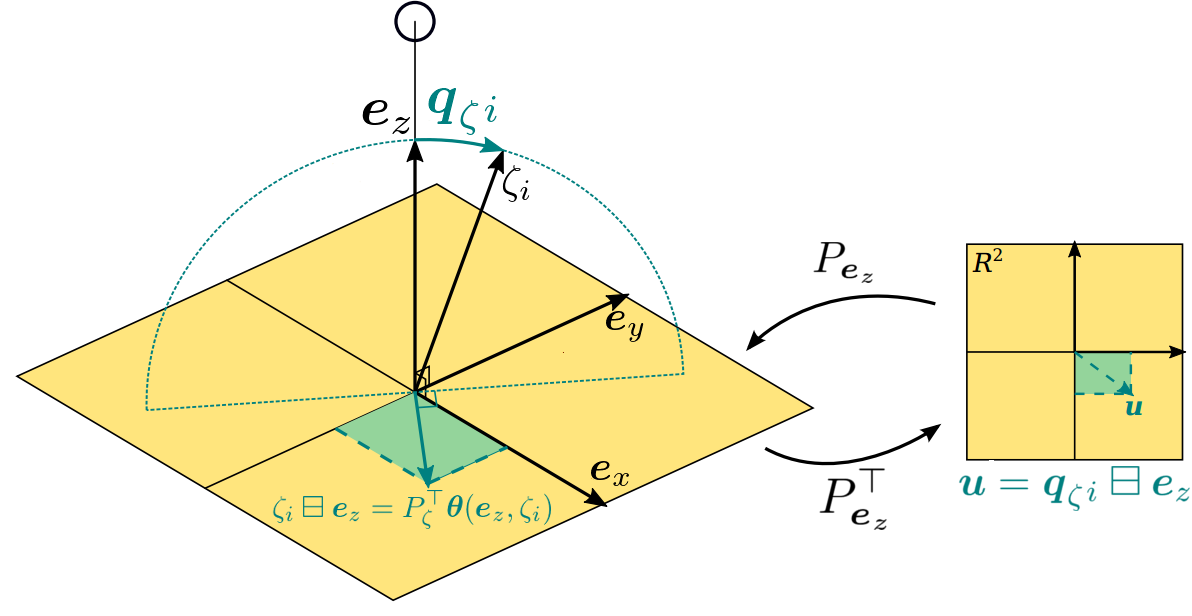
\includegraphics[width=0.8\columnwidth]{figures/unit_vector_picture}
\par\end{centering}

\caption{Illustration of Bearing Vector Geometry}
\end{figure}


As can be seen in the picture, there is only 2 degrees of freedom
in this paramterization, but we are using a quaternion, in $\mathbb{R}^{4}$to
define it. Here are the definitions of the $\boxplus$ and $\boxminus$
operators.

\begin{align}
\boxplus & :SO\left(3\right)\times\mathbb{R}^{2}\rightarrow SO\left(3\right),\\
 & {\bf q_{\zeta}},\boldsymbol{u}\mapsto\exp(P_{\boldsymbol{\zeta}}u)\otimes\boldsymbol{q}_{\zeta},\\
\boxminus & :SO\left(3\right)\times SO\left(3\right)\rightarrow\mathbb{R}^{2},\\
 & {\bf q},{\bf p}\mapsto P_{\boldsymbol{p}}^{\top}\boldsymbol{\theta}\left(n\left(\boldsymbol{p}\right),\:n\left(\boldsymbol{q}\right)\right),
\end{align}


where $\boldsymbol{\theta}$ maps two unit vectors to the minimal
rotation vector between them

\begin{equation}
\boldsymbol{\theta}\left(n\left(\boldsymbol{p}\right),\:n\left(\boldsymbol{q}\right)\right):=\cos^{-1}\left(n\left(\boldsymbol{p}\right)^{\top}n\left(\boldsymbol{q}\right)\right)\dfrac{n\left(\boldsymbol{p}\right)\times n\left(\boldsymbol{q}\right)}{\lVert n\left(\boldsymbol{p}\right)\times n\left(\boldsymbol{q}\right)\rVert}
\end{equation}


and $n\left(\boldsymbol{q}\right)$ is the unit vector which results
when rotating $\boldsymbol{e}_{z}$ by $\boldsymbol{q}$. For example:
\begin{equation}
n(\boldsymbol{q_{\zeta}})=\boldsymbol{\zeta}
\end{equation}



\section{Dynamics}

Now that we have defined all the relevant parameterizations, we can
define the dynamics for our system. We will use generic rigid-body
dynamics mechanized by acceleration and angular velocity inputs $\hat{{\bf a}}$
and $\hat{\boldsymbol{\omega}}$ respectively. We also do everything
in a robo-centric frame


\subsection{Position Dynamics}

The relationship between the inertial and body coordinate systems
defined in the body frame is given by

\begin{align}
_{\mathcal{B}}\dot{{\bf p}}_{\mathcal{B}\mathcal{I}} & =-\dot{R}\left({\bf q}_{\mathcal{B}\mathcal{I}}\right){}_{\mathcal{I}}{\bf p}_{\mathcal{I}\mathcal{B}}-R\left({\bf q}_{\mathcal{B}\mathcal{I}}\right){}_{\mathcal{I}}\dot{{\bf p}}_{\mathcal{I}\mathcal{B}}\\
 & =\left\lfloor _{\mathcal{B}}\boldsymbol{\omega}_{\mathcal{B}\mathcal{I}}\right\rfloor R\left({\bf q}_{\mathcal{B}\mathcal{I}}\right){}_{\mathcal{I}}{\bf p}_{\mathcal{I}\mathcal{B}}-R\left({\bf q}_{\mathcal{B}\mathcal{I}}\right){}_{\mathcal{I}}{\bf v}_{\mathcal{B}\mathcal{I}}\\
 & =\left\lfloor _{\mathcal{B}}\boldsymbol{\omega}_{\mathcal{B}\mathcal{I}}\right\rfloor {}_{\mathcal{B}}{\bf p}_{\mathcal{I}\mathcal{B}}-{}_{\mathcal{B}}{\bf v}_{\mathcal{B}\mathcal{I}}\\
 & =-\left\lfloor _{\mathcal{B}}\boldsymbol{\omega}_{\mathcal{B}\mathcal{I}}\right\rfloor {}_{\mathcal{B}}{\bf p}_{\mathcal{B}\mathcal{I}}-{}_{\mathcal{B}}{\bf v}_{\mathcal{B}\mathcal{I}}.
\end{align}



\subsection{Attitude Dynamics}

From page 34 of \cite{key-4}, the time derivative of attitude is
given by

\begin{align}
\dot{{\bf q}}_{\mathcal{I}\mathcal{B}} & =-_{\mathcal{I}}\boldsymbol{\omega}_{\mathcal{B}\mathcal{I}}\\
 & =-R\left({\bf q}_{\mathcal{I}\mathcal{B}}\right){}_{\mathcal{B}}\boldsymbol{\omega}_{\mathcal{B}\mathcal{I}}.
\end{align}



\subsection{Velocity Dynamics}

Applying Newton's law, we have

\begin{align}
_{\mathcal{B}}{\bf f}+mR^{\top}\left({\bf q}_{\mathcal{I}\mathcal{B}}\right){}_{\mathcal{I}}{\bf g} & =m_{\mathcal{B}}\dot{{\bf v}}_{\mathcal{I}\mathcal{B}}\\
_{\mathcal{B}}{\bf f}+mR^{\top}\left({\bf q}_{\mathcal{I}\mathcal{B}}\right){}_{\mathcal{I}}{\bf g} & =m\left(R^{\top}\left({\bf q}_{\mathcal{I}\mathcal{B}}\right){}_{\mathcal{I}}\dot{{\bf v}}_{\mathcal{B}\mathcal{I}}+\left\lfloor _{\mathcal{B}}\boldsymbol{\omega}_{\mathcal{I}\mathcal{B}}\right\rfloor {}_{\mathcal{B}}{\bf v}_{\mathcal{I}\mathcal{B}}\right)\\
\frac{1}{m}{}_{\mathcal{B}}{\bf f}+R^{\top}\left({\bf q}_{\mathcal{I}\mathcal{B}}\right){}_{\mathcal{I}}{\bf g} & =R^{\top}\left({\bf q}_{\mathcal{I}\mathcal{B}}\right){}_{\mathcal{I}}\dot{{\bf v}}_{\mathcal{B}\mathcal{I}}+\left\lfloor _{\mathcal{B}}\boldsymbol{\omega}_{\mathcal{I}\mathcal{B}}\right\rfloor {}_{\mathcal{B}}{\bf v}_{\mathcal{I}\mathcal{B}}\\
\frac{1}{m}{}_{\mathcal{B}}{\bf f}+R^{\top}\left({\bf q}_{\mathcal{I}\mathcal{B}}\right){}_{\mathcal{I}}{\bf g} & =_{\mathcal{B}}\dot{{\bf v}}_{\mathcal{B}\mathcal{I}}+\left\lfloor _{\mathcal{B}}\boldsymbol{\omega}_{\mathcal{I}\mathcal{B}}\right\rfloor {}_{\mathcal{B}}{\bf v}_{\mathcal{I}\mathcal{B}}\\
_{\mathcal{B}}\dot{{\bf v}}_{\mathcal{B}\mathcal{I}} & =\frac{1}{m}{}_{\mathcal{B}}{\bf f}+R^{\top}\left({\bf q}_{\mathcal{I}\mathcal{B}}\right){}_{\mathcal{I}}{\bf g}-\left\lfloor _{\mathcal{B}}\boldsymbol{\omega}_{\mathcal{I}\mathcal{B}}\right\rfloor {}_{\mathcal{B}}{\bf v}_{\mathcal{I}\mathcal{B}}\\
_{\mathcal{B}}\dot{{\bf v}}_{\mathcal{B}\mathcal{I}} & =_{\mathcal{B}}{\bf a}_{\mathcal{B}\mathcal{I}}+R^{\top}\left({\bf q}_{\mathcal{I}\mathcal{B}}\right){}_{\mathcal{I}}{\bf g}-\left\lfloor _{\mathcal{B}}\boldsymbol{\omega}_{\mathcal{B}\mathcal{I}}\right\rfloor {}_{\mathcal{B}}{\bf v}_{\mathcal{B}\mathcal{I}}.
\end{align}



\subsection{Feature Bearing Vector Dynamics}

We will derive the feature dynamics relative to the camera. A fixed
feature location can be defined in the inertial frame by

\begin{equation}
_{\mathcal{I}}{\bf p}_{\mathcal{I}F}={}_{\mathcal{I}}{\bf p}_{\mathcal{I}\mathcal{C}}+R\left({\bf q}_{\mathcal{I}\mathcal{C}}\right){}_{\mathcal{C}}\boldsymbol{\zeta}_{\mathcal{C}F}d\left(\rho\right).
\end{equation}


Taking the time derivative of the entire equation yields

\begin{align}
0 & =_{\mathcal{I}}{\bf v}_{\mathcal{C}\mathcal{I}}+\frac{d}{dt}\left(R\left({\bf q}_{\mathcal{I}\mathcal{C}}\right)\right){}_{\mathcal{C}}\boldsymbol{\zeta}_{\mathcal{C}F}d\left(\rho\right)+R\left({\bf q}_{\mathcal{I}\mathcal{C}}\right)\frac{d}{dt}\left(_{\mathcal{C}}\boldsymbol{\zeta}_{\mathcal{C}F}\right)d\left(\rho\right)+R\left({\bf q}_{\mathcal{I}\mathcal{C}}\right){}_{\mathcal{C}}\boldsymbol{\zeta}_{\mathcal{C}F}\frac{d}{dt}\left(d\left(\rho\right)\right)\\
 & =_{\mathcal{I}}{\bf v}_{\mathcal{C}\mathcal{I}}+R\left({\bf q}_{\mathcal{I}\mathcal{C}}\right)\left\lfloor _{\mathcal{C}}\boldsymbol{\omega}_{\mathcal{C}\mathcal{I}}\right\rfloor {}_{\mathcal{C}}\boldsymbol{\zeta}_{\mathcal{C}F}d\left(\rho\right)+R\left({\bf q}_{\mathcal{I}\mathcal{C}}\right)\left\lfloor _{\mathcal{C}}\boldsymbol{\zeta}_{\mathcal{C}F}\right\rfloor P_{\zeta}{}_{\mathcal{C}}\dot{\boldsymbol{\zeta}}_{\mathcal{C}F}d\left(\rho\right)+R\left({\bf q}_{\mathcal{I}\mathcal{C}}\right){}_{\mathcal{C}}\boldsymbol{\zeta}_{\mathcal{C}F}d^{\prime}\left(\rho\right)\dot{\rho},
\end{align}
and rotating into the camera frame gives

\begin{align}
0 & =_{\mathcal{C}}{\bf v}_{\mathcal{C}\mathcal{I}}+\left\lfloor _{\mathcal{C}}\boldsymbol{\omega}_{\mathcal{C}\mathcal{I}}\right\rfloor {}_{\mathcal{C}}\boldsymbol{\zeta}_{\mathcal{C}F}d\left(\rho\right)+\left\lfloor _{\mathcal{C}}\boldsymbol{\zeta}_{\mathcal{C}F}\right\rfloor P_{\zeta}{}_{\mathcal{C}}\dot{\boldsymbol{\zeta}}_{\mathcal{C}F}d\left(\rho\right)+{}_{\mathcal{C}}\boldsymbol{\zeta}_{\mathcal{C}F}d^{\prime}\left(\rho\right)\dot{\rho}\\
 & =_{\mathcal{C}}{\bf v}_{\mathcal{C}\mathcal{I}}-\left\lfloor _{\mathcal{C}}\boldsymbol{\zeta}_{\mathcal{C}F}\right\rfloor {}_{\mathcal{C}}\boldsymbol{\omega}_{\mathcal{C}\mathcal{I}}d\left(\rho\right)+\left\lfloor _{\mathcal{C}}\boldsymbol{\zeta}_{\mathcal{C}F}\right\rfloor P_{\zeta}{}_{\mathcal{C}}\dot{\boldsymbol{\zeta}}_{\mathcal{C}F}d\left(\rho\right)+{}_{\mathcal{C}}\boldsymbol{\zeta}_{\mathcal{C}F}d^{\prime}\left(\rho\right)\dot{\rho}.\label{eq:feature}
\end{align}


In order to isolate $_{\mathcal{C}}\dot{\boldsymbol{\zeta}}_{\mathcal{C}F}$,
multiply by $d\left(\rho\right)^{-1}P_{\zeta}^{\top}\left\lfloor _{\mathcal{C}}\boldsymbol{\zeta}_{\mathcal{C}F}\right\rfloor $
to get

\begin{align}
0 & =d\left(\rho\right)^{-1}P_{\zeta}^{\top}\left\lfloor _{\mathcal{C}}\boldsymbol{\zeta}_{\mathcal{C}F}\right\rfloor {}_{\mathcal{C}}{\bf v}_{\mathcal{C}\mathcal{I}}-d\left(\rho\right)^{-1}P_{\zeta}^{\top}\left\lfloor _{\mathcal{C}}\boldsymbol{\zeta}_{\mathcal{C}F}\right\rfloor \left\lfloor _{\mathcal{C}}\boldsymbol{\zeta}_{\mathcal{C}F}\right\rfloor {}_{\mathcal{C}}\boldsymbol{\omega}_{\mathcal{C}\mathcal{I}}d\left(\rho\right)+d\left(\rho\right)^{-1}P_{\zeta}^{\top}\left\lfloor _{\mathcal{C}}\boldsymbol{\zeta}_{\mathcal{C}F}\right\rfloor \left\lfloor _{\mathcal{C}}\boldsymbol{\zeta}_{\mathcal{C}F}\right\rfloor P_{\zeta}{}_{\mathcal{C}}\dot{\boldsymbol{\zeta}}_{\mathcal{C}F}d\left(\rho\right)+d\left(\rho\right)^{-1}P_{\zeta}^{\top}\left\lfloor _{\mathcal{C}}\boldsymbol{\zeta}_{\mathcal{C}F}\right\rfloor {}_{\mathcal{C}}\boldsymbol{\zeta}_{\mathcal{C}F}d^{\prime}\left(\rho\right)\dot{\rho}\\
 & =d\left(\rho\right)^{-1}P_{\zeta}^{\top}\left\lfloor _{\mathcal{C}}\boldsymbol{\zeta}_{\mathcal{C}F}\right\rfloor {}_{\mathcal{C}}{\bf v}_{\mathcal{C}\mathcal{I}}-P_{\zeta}^{\top}\left\lfloor _{\mathcal{C}}\boldsymbol{\zeta}_{\mathcal{C}F}\right\rfloor \left\lfloor _{\mathcal{C}}\boldsymbol{\zeta}_{\mathcal{C}F}\right\rfloor {}_{\mathcal{C}}\boldsymbol{\omega}_{\mathcal{C}\mathcal{I}}+P_{\zeta}^{\top}\left\lfloor _{\mathcal{C}}\boldsymbol{\zeta}_{\mathcal{C}F}\right\rfloor \left\lfloor _{\mathcal{C}}\boldsymbol{\zeta}_{\mathcal{C}F}\right\rfloor P_{\zeta}{}_{\mathcal{C}}\dot{\boldsymbol{\zeta}}_{\mathcal{C}F},
\end{align}
and using the identity $P_{\zeta}^{\top}\left\lfloor _{\mathcal{C}}\boldsymbol{\zeta}_{\mathcal{C}F}\right\rfloor \left\lfloor _{\mathcal{C}}\boldsymbol{\zeta}_{\mathcal{C}F}\right\rfloor =-P_{\zeta}^{\top}$
followed by $P_{\zeta}^{\top}P_{\zeta}=I$ gives us

\begin{align}
0 & =d\left(\rho\right)^{-1}P_{\zeta}^{\top}\left\lfloor _{\mathcal{C}}\boldsymbol{\zeta}_{\mathcal{C}F}\right\rfloor {}_{\mathcal{C}}{\bf v}_{\mathcal{C}\mathcal{I}}+P_{\zeta}^{\top}{}_{\mathcal{C}}\boldsymbol{\omega}_{\mathcal{C}\mathcal{I}}-P_{\zeta}^{\top}P_{\zeta}{}_{\mathcal{C}}\dot{\boldsymbol{\zeta}}_{\mathcal{C}F}\\
 & =d\left(\rho\right)^{-1}P_{\zeta}^{\top}\left\lfloor _{\mathcal{C}}\boldsymbol{\zeta}_{\mathcal{C}F}\right\rfloor {}_{\mathcal{C}}{\bf v}_{\mathcal{C}\mathcal{I}}+P_{\zeta}^{\top}{}_{\mathcal{C}}\boldsymbol{\omega}_{\mathcal{C}\mathcal{I}}-{}_{\mathcal{C}}\dot{\boldsymbol{\zeta}}_{\mathcal{C}F}.
\end{align}


Solving for $_{\mathcal{C}}\dot{\boldsymbol{\zeta}}_{\mathcal{C}F}$
yields

\begin{align}
_{\mathcal{C}}\dot{\boldsymbol{\zeta}}_{\mathcal{C}F} & =P_{\zeta}^{\top}\left(_{\mathcal{C}}\boldsymbol{\omega}_{\mathcal{C}\mathcal{I}}+\left\lfloor _{\mathcal{C}}\boldsymbol{\zeta}_{\mathcal{C}F}\right\rfloor \frac{_{\mathcal{C}}{\bf v}_{\mathcal{C}\mathcal{I}}}{d\left(\rho\right)}\right)\\
 & =P_{\zeta}^{\top}\left(_{\mathcal{C}}\boldsymbol{\omega}_{\mathcal{C}\mathcal{I}}+\rho\left\lfloor _{\mathcal{C}}\boldsymbol{\zeta}_{\mathcal{C}F}\right\rfloor {}_{\mathcal{C}}{\bf v}_{\mathcal{C}\mathcal{I}}\right).
\end{align}



\subsection{Feature Distance Dynamics}

Now, to isolate $\dot{\rho}$, multiply \ref{eq:feature} by $d^{\prime}\left(\rho\right)^{-1}{}_{\mathcal{C}}\boldsymbol{\zeta}_{\mathcal{C}F}^{\top}$
to get

\begin{align}
0 & =d^{\prime}\left(\rho\right)^{-1}{}_{\mathcal{C}}\boldsymbol{\zeta}_{\mathcal{C}F}^{\top}{}_{\mathcal{C}}{\bf v}_{\mathcal{C}\mathcal{I}}-d^{\prime}\left(\rho\right)^{-1}{}_{\mathcal{C}}\boldsymbol{\zeta}_{\mathcal{C}F}^{\top}\left\lfloor _{\mathcal{C}}\boldsymbol{\zeta}_{\mathcal{C}F}\right\rfloor {}_{\mathcal{C}}\boldsymbol{\omega}_{\mathcal{C}\mathcal{I}}d\left(\rho\right)+d^{\prime}\left(\rho\right)^{-1}{}_{\mathcal{C}}\boldsymbol{\zeta}_{\mathcal{C}F}^{\top}\left\lfloor _{\mathcal{C}}\boldsymbol{\zeta}_{\mathcal{C}F}\right\rfloor P_{\zeta}{}_{\mathcal{C}}\dot{\boldsymbol{\zeta}}_{\mathcal{C}F}d\left(\rho\right)+d^{\prime}\left(\rho\right)^{-1}{}_{\mathcal{C}}\boldsymbol{\zeta}_{\mathcal{C}F}^{\top}{}_{\mathcal{C}}\boldsymbol{\zeta}_{\mathcal{C}F}d^{\prime}\left(\rho\right)\dot{\rho}\\
 & =d^{\prime}\left(\rho\right)^{-1}{}_{\mathcal{C}}\boldsymbol{\zeta}_{\mathcal{C}F}^{\top}{}_{\mathcal{C}}{\bf v}_{\mathcal{C}\mathcal{I}}+\dot{\rho},
\end{align}
and solving for $\dot{\rho}$ yields

\begin{align}
\dot{\rho} & =\dfrac{_{\mathcal{C}}\boldsymbol{\zeta}_{\mathcal{C}F}^{\top}{}_{\mathcal{C}}{\bf v}_{\mathcal{C}\mathcal{I}}}{d^{\prime}\left(\rho\right)}\\
 & =-\rho^{2}{}_{\mathcal{C}}\boldsymbol{\zeta}_{\mathcal{C}F}^{\top}{}_{\mathcal{C}}{\bf v}_{\mathcal{C}\mathcal{I}}.
\end{align}



\section{Propagation}

Because we are using the $\boxplus$ and $\boxminus$ notation, progation
works as follows under Euler integration:

\begin{align}
\boldsymbol{\hat{x}}\left(t+\Delta t\right) & =\hat{{\bf x}}\left(t\right)\boxplus\dot{\hat{{\bf x}}}\Delta t
\end{align}


For clarity, let's break up the state into three parts, the vector
part, the attitude part and feature bearing vector part.

First the vector portion:

\begin{align}
\hat{{\bf x}}_{{\bf v}}\left(t+\Delta t\right) & =\hat{{\bf x}}_{{\bf v}}\left(t\right)\boxplus\dot{\hat{{\bf x}}}_{{\bf v}}\Delta t\\
 & =\hat{{\bf x}}_{{\bf v}}\left(t\right)+\dot{\hat{{\bf x}}}_{{\bf v}}\Delta t
\end{align}


Then the Attitude quaternion portion 
\begin{align}
\hat{{\bf x}}_{{\bf q}}\left(t+\Delta t\right) & =\hat{{\bf x}}_{{\bf q}}\left(t\right)\boxplus\dot{\hat{{\bf x}}}_{{\bf q}}\Delta t\\
 & =\hat{{\bf x}}_{{\bf q}}\left(t\right)\otimes\exp\left(\dot{\hat{{\bf q}}}\Delta t\right)\\
 & =\hat{{\bf x}}_{{\bf q}}\left(t\right)\otimes\exp\left(-R\left(\hat{{\bf q}}\right)\boldsymbol{\omega}\left(t\right)\Delta t\right)
\end{align}


and finally the bearing vector quaternion portion

\begin{align}
\hat{{\bf x}}_{\boldsymbol{\zeta}_{i}}\left(t+\Delta t\right) & =\hat{{\bf x}}_{\boldsymbol{\zeta}_{i}}\left(t\right)\boxplus\dot{\hat{{\bf x}}}_{\zeta_{i}}\Delta t\\
 & =\exp\left(P_{\hat{\zeta}_{i}}\dot{\boldsymbol{\zeta}_{i}}\Delta t\right)\otimes\hat{{\bf x}}_{\boldsymbol{\zeta}_{i}}\left(t\right)\\
 & =\exp\left(P_{\hat{\zeta}_{i}}\dot{P_{\zeta}^{\top}\left(_{\mathcal{C}}\boldsymbol{\omega}_{\mathcal{C}\mathcal{I}}+\rho\left\lfloor _{\mathcal{C}}\boldsymbol{\zeta}_{\mathcal{C}F}\right\rfloor {}_{\mathcal{C}}{\bf v}_{\mathcal{C}\mathcal{I}}\right)_{i}}\Delta t\right)\otimes\hat{{\bf x}}_{\boldsymbol{\zeta}_{i}}\left(t\right)
\end{align}


The Jacobians are found with respect to the state and input noise
given

\begin{align}
{\bf x} & =\begin{bmatrix}_{\mathcal{B}}{\bf p}_{\mathcal{B}\mathcal{I}}^{\top} & {\bf q}_{\mathcal{I}\mathcal{B}}^{\top} & _{\mathcal{B}}{\bf v}_{\mathcal{B}\mathcal{I}}^{\top} & \boldsymbol{\beta}_{\boldsymbol{\omega}}^{\top} & \boldsymbol{\beta}_{a}^{\top} & {\bf q}_{\zeta}^{\top} & \rho\end{bmatrix}^{\top}\\
{\bf u} & =\begin{bmatrix}\boldsymbol{\eta}_{\omega}^{\top} & \boldsymbol{\eta}_{a}^{\top} & \boldsymbol{\eta}_{\zeta}^{\top} & \eta_{\rho}^{\top}\end{bmatrix}^{\top},
\end{align}


where it's important to recall that $\dot{{\bf q}}_{\mathcal{I}\mathcal{B}}\in\mathbb{R}^{3}$,
$\dot{{\bf q}}_{\mathcal{F}\mathcal{C}}\in\mathbb{R}^{2}$, $\boldsymbol{\eta}_{\zeta}\in\mathbb{R}^{2}$,
and $\eta_{\rho}\in\mathbb{R}$. 


\subsection{Dynamics}

The true body-relative state dynamics with noise added where appropriate
are given by

\begin{align}
_{\mathcal{B}}\dot{{\bf p}}_{\mathcal{B}\mathcal{I}} & =-\left\lfloor _{\mathcal{B}}\boldsymbol{\omega}_{\mathcal{B}\mathcal{I}}\right\rfloor {}_{\mathcal{B}}{\bf p}_{\mathcal{B}\mathcal{I}}-{}_{\mathcal{B}}{\bf v}_{\mathcal{B}\mathcal{I}}\\
\dot{{\bf q}}_{\mathcal{I}\mathcal{B}} & =-R\left({\bf q}_{\mathcal{I}\mathcal{B}}\right){}_{\mathcal{B}}\boldsymbol{\omega}_{\mathcal{B}\mathcal{I}}\\
_{\mathcal{B}}\dot{{\bf v}}_{\mathcal{B}\mathcal{I}} & ={\bf k}{\bf k}^{\top}{}_{\mathcal{B}}{\bf a}_{\mathcal{B}\mathcal{I}}+R^{\top}\left({\bf q}_{\mathcal{I}\mathcal{B}}\right){}_{\mathcal{I}}{\bf g}-\left\lfloor _{\mathcal{B}}\boldsymbol{\omega}_{\mathcal{B}\mathcal{I}}\right\rfloor {}_{\mathcal{B}}{\bf v}_{\mathcal{B}\mathcal{I}}\\
\dot{\boldsymbol{\beta}}_{\omega} & =\boldsymbol{\eta}_{\omega}\\
\dot{\boldsymbol{\beta}}_{a} & =\boldsymbol{\eta}_{a}\\
\dot{{\bf q}}_{\mathcal{F}\mathcal{C}} & =P_{\zeta}^{\top}\left(_{\mathcal{C}}\boldsymbol{\omega}_{\mathcal{C}\mathcal{I}}+\rho\left\lfloor _{\mathcal{C}}\boldsymbol{\zeta}_{\mathcal{C}F}\right\rfloor {}_{\mathcal{C}}{\bf v}_{\mathcal{C}\mathcal{I}}\right)+\boldsymbol{\eta}_{\zeta}\\
\dot{\rho} & =-\rho^{2}{}_{\mathcal{C}}\boldsymbol{\zeta}_{\mathcal{C}F}^{\top}{}_{\mathcal{C}}{\bf v}_{\mathcal{C}\mathcal{I}}+\eta_{\rho},
\end{align}


where

\begin{align}
_{\mathcal{B}}\boldsymbol{\omega}_{\mathcal{B}\mathcal{I}} & =_{\mathcal{B}}\bar{\boldsymbol{\omega}}_{\mathcal{B}\mathcal{I}}-\boldsymbol{\beta}_{\omega}-\boldsymbol{\eta}_{\omega}\\
_{\mathcal{B}}{\bf a}_{\mathcal{B}\mathcal{I}} & =_{\mathcal{B}}\bar{{\bf a}}_{\mathcal{B}\mathcal{I}}-\boldsymbol{\beta}_{a}-\boldsymbol{\eta}_{a}.
\end{align}



\subsection{Jacobians}

The Jacobian of the state dynamics w.r.t. the state is then given
by

\begin{equation}
F=\dfrac{\partial\dot{{\bf x}}}{\partial{\bf x}}=\begin{bmatrix}-\left\lfloor _{\mathcal{B}}\boldsymbol{\omega}_{\mathcal{B}\mathcal{I}}\right\rfloor  & {\bf 0} & -I & -\left\lfloor _{\mathcal{B}}{\bf p}_{\mathcal{B}\mathcal{I}}\right\rfloor  & {\bf 0} & {\bf 0} & {\bf 0}\\
{\bf 0} & \left\lfloor R\left({\bf q}_{\mathcal{I}\mathcal{B}}\right){}_{\mathcal{B}}\boldsymbol{\omega}_{\mathcal{B}\mathcal{I}}\right\rfloor  & {\bf 0} & R\left({\bf q}_{\mathcal{I}\mathcal{B}}\right) & {\bf 0} & {\bf 0} & {\bf 0}\\
{\bf 0} & -\left\lfloor R^{\top}\left({\bf q}_{\mathcal{I}\mathcal{B}}\right){}_{\mathcal{I}}{\bf g}\right\rfloor  & -\left\lfloor _{\mathcal{B}}\boldsymbol{\omega}_{\mathcal{B}\mathcal{I}}\right\rfloor  & -\left\lfloor _{\mathcal{B}}{\bf v}_{\mathcal{B}\mathcal{I}}\right\rfloor  & -{\bf k}{\bf k}^{\top} & {\bf 0} & {\bf 0}\\
{\bf 0} & {\bf 0} & {\bf 0} & {\bf 0} & {\bf 0} & {\bf 0} & {\bf 0}\\
{\bf 0} & {\bf 0} & {\bf 0} & {\bf 0} & {\bf 0} & {\bf 0} & {\bf 0}\\
{\bf 0} & {\bf 0} & \dfrac{\partial\dot{{\bf q}}_{\mathcal{I}\mathcal{B}}}{\partial{}_{\mathcal{B}}{\bf v}_{\mathcal{B}\mathcal{I}}} & \dfrac{\partial\dot{{\bf q}}_{\mathcal{I}\mathcal{B}}}{\partial\boldsymbol{\beta}_{\omega}} & {\bf 0} & \dfrac{\partial\dot{{\bf q}}_{\mathcal{I}\mathcal{B}}}{\partial{\bf q}_{\zeta}} & \dfrac{\partial\dot{{\bf q}}_{\mathcal{I}\mathcal{B}}}{\partial\rho}\\
{\bf 0} & {\bf 0} & \dfrac{\partial\dot{\rho}}{\partial{}_{\mathcal{B}}{\bf v}_{\mathcal{B}\mathcal{I}}} & \dfrac{\partial\dot{\rho}}{\partial\boldsymbol{\beta}_{\omega}} & {\bf 0} & \dfrac{\partial\dot{\rho}}{\partial{\bf q}_{\zeta}} & \dfrac{\partial\dot{\rho}}{\partial\rho}
\end{bmatrix},
\end{equation}


where

\begin{align}
\dfrac{\partial\dot{{\bf q}}_{\mathcal{I}\mathcal{B}}}{\partial{}_{\mathcal{B}}{\bf v}_{\mathcal{B}\mathcal{I}}} & =\rho P_{\zeta}^{\top}\left\lfloor _{\mathcal{C}}\boldsymbol{\zeta}_{\mathcal{C}F}\right\rfloor R\left({\bf q}_{\mathcal{C}\mathcal{B}}\right)\\
\dfrac{\partial\dot{{\bf q}}_{\mathcal{I}\mathcal{B}}}{\partial\boldsymbol{\beta}_{\omega}} & =P_{\zeta}^{\top}\left(-R\left({\bf q}_{\mathcal{C}\mathcal{B}}\right)+\rho\left\lfloor _{\mathcal{C}}\boldsymbol{\zeta}_{\mathcal{C}F}\right\rfloor R\left({\bf q}_{\mathcal{C}\mathcal{B}}\right)\left\lfloor _{\mathcal{B}}{\bf p}_{\mathcal{B}\mathcal{C}}\right\rfloor \right)\\
\dfrac{\partial\dot{{\bf q}}_{\mathcal{I}\mathcal{B}}}{\partial{\bf q}_{\zeta}} & =-P_{\zeta}^{\top}\left\lfloor _{\mathcal{C}}\boldsymbol{\omega}_{\mathcal{C}\mathcal{I}}\right\rfloor P_{\zeta}-\rho\dfrac{\partial}{\partial{\bf q}_{\zeta}}\left(P_{\zeta}^{\top}\left\lfloor _{\mathcal{C}}{\bf v}_{\mathcal{C}\mathcal{I}}\right\rfloor {}_{\mathcal{C}}\boldsymbol{\zeta}_{\mathcal{C}F}\right)\\
\dfrac{\partial\dot{{\bf q}}_{\mathcal{I}\mathcal{B}}}{\partial\rho} & =P_{\zeta}^{\top}\left\lfloor _{\mathcal{C}}\boldsymbol{\zeta}_{\mathcal{C}F}\right\rfloor {}_{\mathcal{C}}{\bf v}_{\mathcal{C}\mathcal{I}}\\
\dfrac{\partial\dot{\rho}}{\partial{}_{\mathcal{B}}{\bf v}_{\mathcal{B}\mathcal{I}}} & =-\rho^{2}{}_{\mathcal{C}}\boldsymbol{\zeta}_{\mathcal{C}F}^{\top}R\left({\bf q}_{\mathcal{C}\mathcal{B}}\right)\\
\dfrac{\partial\dot{\rho}}{\partial\boldsymbol{\beta}_{\omega}} & =-\rho^{2}{}_{\mathcal{C}}\boldsymbol{\zeta}_{\mathcal{C}F}^{\top}R\left({\bf q}_{\mathcal{C}\mathcal{B}}\right)\left\lfloor _{\mathcal{B}}{\bf p}_{\mathcal{B}\mathcal{C}}\right\rfloor \\
\dfrac{\partial\dot{\rho}}{\partial{\bf q}_{\zeta}} & =-\rho^{2}{}_{\mathcal{C}}{\bf v}_{\mathcal{C}\mathcal{I}}^{\top}\left\lfloor _{\mathcal{C}}\boldsymbol{\zeta}_{\mathcal{C}F}\right\rfloor P_{\zeta}\\
\dfrac{\partial\dot{\rho}}{\partial\rho} & =-2\rho{}_{\mathcal{C}}\boldsymbol{\zeta}_{\mathcal{C}F}^{\top}{}_{\mathcal{C}}{\bf v}_{\mathcal{C}\mathcal{I}}.
\end{align}


The Jacobian of the state dynamics w.r.t. the input noise is given
by

\begin{equation}
G=\dfrac{\partial\dot{{\bf x}}}{\partial{\bf u}}=\begin{bmatrix}-\left\lfloor _{\mathcal{B}}{\bf p}_{\mathcal{B}\mathcal{I}}\right\rfloor  & {\bf 0} & {\bf 0} & {\bf 0}\\
R\left({\bf q}_{\mathcal{I}\mathcal{B}}\right) & {\bf 0} & {\bf 0} & {\bf 0}\\
-\left\lfloor _{\mathcal{B}}{\bf v}_{\mathcal{B}\mathcal{I}}\right\rfloor  & -{\bf k}{\bf k}^{\top} & {\bf 0} & {\bf 0}\\
I & {\bf 0} & {\bf 0} & {\bf 0}\\
{\bf 0} & I & {\bf 0} & {\bf 0}\\
\dfrac{\partial\dot{\boldsymbol{\zeta}}}{\partial\boldsymbol{\eta}_{\omega}} & {\bf 0} & I & {\bf 0}\\
\dfrac{\partial\dot{\rho}}{\partial\boldsymbol{\eta}_{\omega}} & {\bf 0} & {\bf 0} & 1
\end{bmatrix},
\end{equation}


where

\begin{align}
\dfrac{\partial\dot{{\bf q}}_{\zeta}}{\partial\boldsymbol{\eta}_{\omega}} & =P_{\zeta}^{\top}\left(-R\left({\bf q}_{\mathcal{C}\mathcal{B}}\right)+\rho\left\lfloor _{\mathcal{C}}\boldsymbol{\zeta}_{\mathcal{C}F}\right\rfloor R\left({\bf q}_{\mathcal{C}\mathcal{B}}\right)\left\lfloor _{\mathcal{B}}{\bf p}_{\mathcal{B}\mathcal{C}}\right\rfloor \right)\\
\dfrac{\partial\dot{\rho}}{\partial\boldsymbol{\eta}_{\omega}} & =-\rho^{2}{}_{\mathcal{C}}\boldsymbol{\zeta}_{\mathcal{C}F}^{\top}R\left({\bf q}_{\mathcal{C}\mathcal{B}}\right)\left\lfloor _{\mathcal{B}}{\bf p}_{\mathcal{B}\mathcal{C}}\right\rfloor .
\end{align}

\begin{thebibliography}{1}
\bibitem{key-1}Hertzberg, Christoph, et al. \textquotedbl{}Integrating
generic sensor fusion algorithms with sound state representations
through encapsulation of manifolds.\textquotedbl{} Information Fusion
14.1 (2013): 57-77.

\bibitem{key-2}Wheeler and Koch. \textquotedbl{}Derivation of the
Relative Multiplicative Extended Kalman Filter\textquotedbl{}

\bibitem{key-3}Beard, Randal W., and Timothy W. McLain. \textquotedbl{}Small
unmanned aircraft: Theory and practice\textquotedbl{}. Princeton university
press, 2012.

\bibitem{key-4}Bloesch, Michael Andre. State Estimation for Legged
Robots\textendash Kinematics, Inertial Sensing, and Computer Vision.
Diss. 2017.\end{thebibliography}

\end{document}
